\documentclass{beamer}

% 主题设置
\usetheme{Madrid}
\usepackage[authoryear, round]{natbib} % 引用 natbib 包,并设置为 authoryear 样式
\usepackage{xeCJK}
\setCJKmainfont{SimSun}
\usepackage{graphicx}
\usepackage{subfigure}
\usepackage{amsmath}
\usepackage{amssymb}

% 页面信息
\title{动力系统模型及其在实时血糖预测中的应用}
\author{刘益通}
\institute{上海科技大学}
\date{\today}
\logo{
\includegraphics[height=0.8cm]{Img/ShanghaiTech_Logo.png}}
\begin{document}

\AtBeginSection[]{
  \begin{frame}
    \frametitle{目录}
    \tableofcontents[currentsection]
  \end{frame}
}

% 标题页
\begin{frame}
  \titlepage
\end{frame}

% 目录页
\begin{frame}
  \frametitle{目录}
  \tableofcontents
\end{frame}

% 第一部分
\section{研究背景}
\begin{frame}
  \frametitle{研究背景}
    WHO数据显示,全球有4.25亿糖尿病患者,占全球人口的8.5\%,而且这个数字还在不断增长。糖尿病问题已经成为全球性的公共卫生问题。CGM技术的发展为糖尿病患者提供了一种实时监测血糖的方法,但是如何利用这些数据进行血糖预测仍然是一个挑战。
\end{frame}

\begin{frame}
  \frametitle{研究目标}
    目前现有的血糖预测动力系统模型大多是基于生物反馈系统的理论,这些模型并没有足够的数据支撑,本文尝试利用CGM采集的大量数据,进行模型拟合,以此验证模型的有效性,之后尝试使用拟合的模型进行实时血糖预测。
\end{frame}

\section{动力系统模型}

\begin{frame}
    \frametitle{动力系统模型基础理论}
    动力系统模型是描述一个系统的状态随时间演化的数学模型,主要通过一组微分方程或差分方程来描述系统的动态行为。

    本文主要使用的动力系统模型是由Best等人提出的葡萄糖-胰岛素动力系统模型\cite{best1981glucose}以及后续发展的胰$\beta$细胞动力系统模型\cite{topp2000model}。
\end{frame}
\begin{frame}
  \frametitle{葡萄糖动力系统}
  \begin{equation}\label{1}
    \frac{dG}{dt} = \text{Production} - \text{Uptake},
\end{equation}
其中$G$是血液中的葡萄糖浓度,$t$是时间,Production是葡萄糖生成速率,Uptake是葡萄糖摄取速率(也可以理解为血液中葡萄糖的消耗速率)。
\end{frame}

\begin{frame}
    \frametitle{葡萄糖动力系统}
    因此,我们可以将葡萄糖产生和摄取速率表示为\cite{best1981glucose}:

\begin{equation}\label{2}
    \text{Production} = P_0 -(E_{G0P} + S_{IP} \times I) \times G,
\end{equation}
\begin{equation}\label{3}
    \text{Uptake} = U_0 + (E_{G0U} + S_{IU} \times I) \times G,
\end{equation}

其中$P_0$和$U_0$是零葡萄糖时的葡萄糖产生和摄取速率,\(E_{G0P}\)和\(E_{G0U}\)分别是产生和摄取的零胰岛素葡萄糖效力,\(S_{IP}\)和\(S_{IU}\)分别是产生和摄取的胰岛素敏感性,$I$代表血胰岛素浓度。
    

\end{frame}

\begin{frame}
    \frametitle{葡萄糖动力系统}
    将方程(\ref{2})和(\ref{3})代入方程(\ref{1}),我们得到

\begin{equation}
    \frac{dG}{dt} = R_0 -(E_{G0} + S_I \times I) \times G,
\end{equation}
其中$R_0$($=P_0-U_0$)是零葡萄糖时葡萄糖的净产生速率,\(E_{G0}\)($=E_{G0p}+E_{G0U}$)是零胰岛素时的总葡萄糖效力,\(S_I\)($=S_{IP}-S_{IU}$)是总胰岛素敏感性。
\end{frame}

\begin{frame}
    \frametitle{胰岛素动力系统}
    类似的,我们可以通过以下微分方程来描述胰岛素动力系统:

    \begin{equation}\label{4}
        \frac{dI}{dt} = \text{Secretion} - \text{Clearance},
    \end{equation}
    其中Secretion表示胰岛素分泌速率,Clearance表示胰岛素清除速率。
    

\end{frame}

\begin{frame}
    \frametitle{胰岛素动力系统}
    我们得到:
    \begin{equation}
        \frac{dI}{dt} = \frac{\beta\sigma G^2}{(\alpha + G^2)} - kI.
    \end{equation}
    其中$k$是代表肝脏、肾脏和胰岛素受体中胰岛素摄取的清除常数,$\beta$是胰$\beta$细胞的质量。所有$\beta$细胞被假定以相同的最大速率$\sigma$分泌胰岛素。$\alpha$是控制S形函数的参数\cite{topp2000model}。  

\end{frame}

\begin{frame}
    \frametitle{胰$\beta$细胞动力系统}
    我们可以通过以下微分方程来描述胰$\beta$细胞动力系统:
    \begin{equation}
        \frac{d\beta}{dt} = (-d_0+r_1G-r_2G^2)\beta,
    \end{equation}
    
    其中$d_0$是零血糖时$\beta$细胞的自然死亡率,$r_1$和$r_2$是两个常系数\cite{topp2000model}。
    

\end{frame}
% 第四部分
\section{模型拟合与预测}
\begin{frame}
  \frametitle{模型拟合}
  \begin{enumerate}
    \item 预处理CGM数据
    \item 将动力系统模型离散化为差分方程形式
    \begin{equation}
        \begin{aligned}
            G_{t+1} & = G_t + 2\Delta t(a_0-a_1G_t-a_2G_tI_t),  \\
            I_{t+1} & = I_t + 2\Delta t(\frac{b_1 G_t^2}{G_t^2 + b_2^2} - b_3 I_t),
        \end{aligned}
    \end{equation}
    \item 使用梯度下降法拟合模型参数
  \end{enumerate}
\end{frame}

\begin{frame}
    \frametitle{拟合结果}
    \begin{figure}[H]
        \centering
        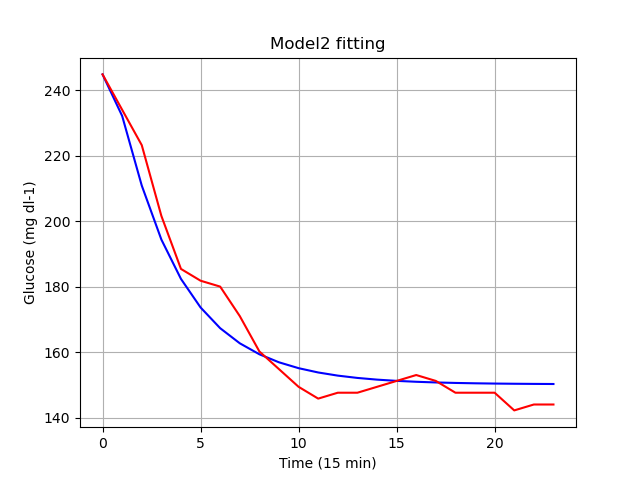
\includegraphics[width=0.7\textwidth]{Img/fit.png}
        \caption{模型拟合结果。}
    \end{figure}
\end{frame}

\begin{frame}
    \frametitle{预测结果}
    \begin{figure}[H]
        \centering
        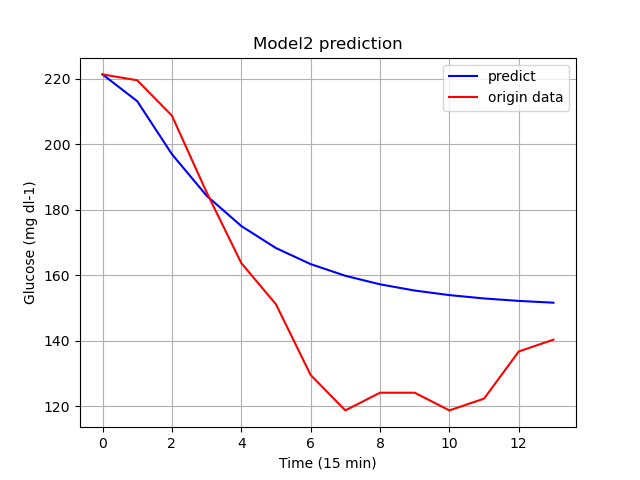
\includegraphics[width=0.7\textwidth]{Img/predict.png}
        \caption{模型预测效果。}
    \end{figure}
\end{frame}

\section{结论与展望}
\begin{frame}
    \frametitle{结论与展望}
    \begin{figure}[H]
        \begin{minipage}[t]{0.4\textwidth}
            \centering
            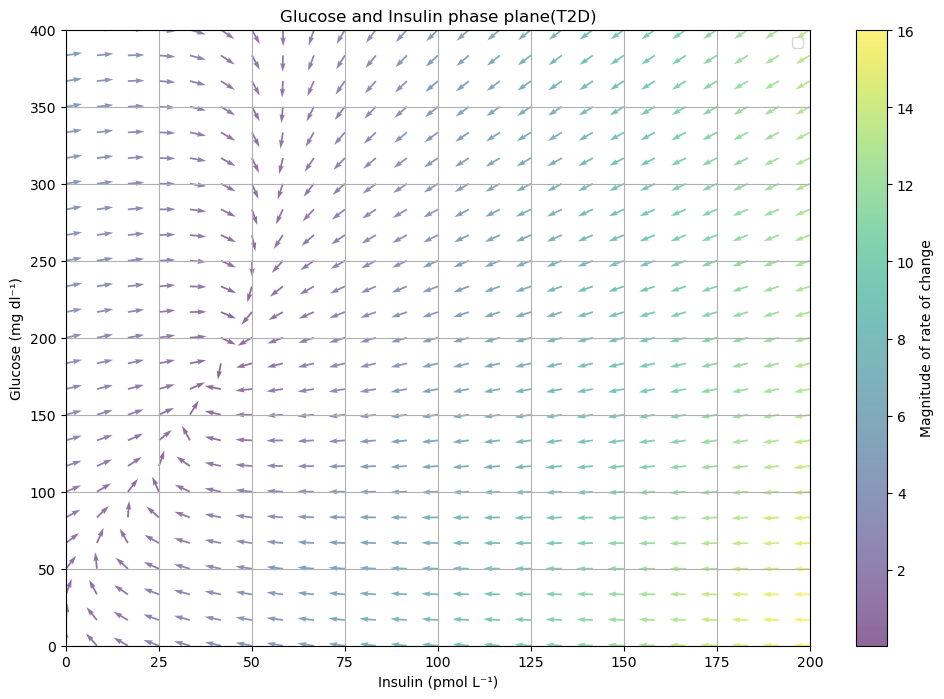
\includegraphics[width=0.9\textwidth]{Img/t2dphase.png}
        \end{minipage}
        \begin{minipage}[t]{0.4\textwidth}
            \centering
            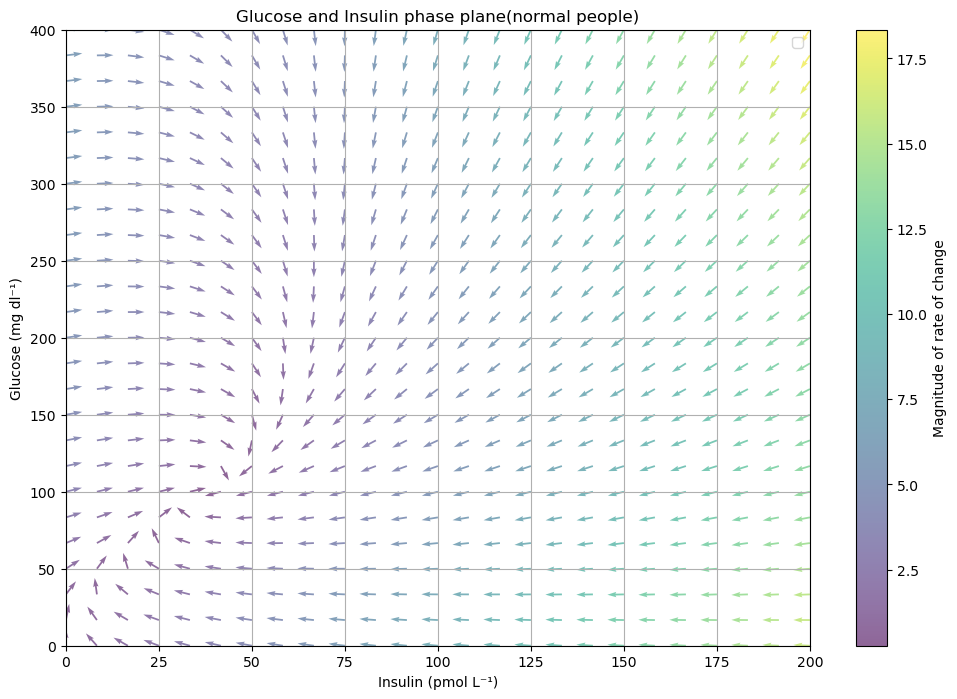
\includegraphics[width=0.9\textwidth]{Img/normalphase.png}
        \end{minipage}
        \caption{2型糖尿病病人与正常人拟合的模型相图差距。}
    \end{figure}
\end{frame}

\begin{frame}
  \frametitle{参考文献}
  \bibliographystyle{plainnat} % 使用 plainnat 样式
  \bibliography{Biblio/ref} % 指定参考文献文件
\end{frame}

\begin{frame}

    \begin{center}
        \huge{请各位老师批评指正!}
    \end{center}

\end{frame}
\end{document}
